\chapter{Summary} % (fold)
\label{cha:summary_&_outlook}
This thesis covers two broader topics: a) The characterisation study of made in India Gas Electron Multiplier (GEM) foil using the electrical and optical characterisation along with the upgrade studies performed for the CMS muon system upgrade using GEM detectors, also known as GE1/1 upgrade. b) physics analysis work performed for the measurement of the anomalous Quartic-Gauge Coupling (aQGC). A brief summary of these task is given below.

On the hardware front, work performed for the upgrade studies of the CMS detector muon endcap system is reported. For the CMS muon endcap detector system upgrade, the Gas Electron Multiplier (GEM) detectors are proposed to be installed during the Long Shutdown-2 (2019-2020) period because of its excellent performance in the harsh running environment like LHC. This upgrade project is named as GE1/1 upgrade, where the letter ``G'' stands for GEM, ``E'' stands for End-cap, the first ``1'' corresponds to the first muon station and the second ``1'' corresponds to the first ring of the station. To test the functionality of these GE1/1 detectors, several beam tests were carried out in 2014 to measure their properties and evaluate their performance in terms of spatial and timing resolution, cluster size and efficiency measurements. It is found that the GE1/1 prototype has efficiency of $>98\%$, time-resolution is $\sim$5-7 ns and space resolution is ~100-100 $\mu m$. Furthermore, with the comparison of the performance of the GE1/1 detectors with the gas mixture of Ar \& $CO_2$ and also Ar, $CO_2$ \& $CF_4$ it is shown that one can operate the GEM detectors without using $CF_4$ gas, which is a non-eco friendly gas, without compromising the efficiency and the time resolution of the detector.

Along with the GE1/1 upgrade studies the characterization studies of the GEM foil developed in India was also performed at the University of Delhi lab. An Indian company, Micropack Pvt. Ltd., got the technology for GEM foil production through the Transfer of Technology (TOT) agreement with CERN. It was successfully able to produce $10~cm~\times~10~cm$ foils using the double mask technique~\cite{DEOLIVEIRA2009}. This GEM foil is characterized using the optical and electrical method. It is found that there are only 0.13\% defects present in the foil and the leakage current is always found to be $<$10 nA, set by CERN quality control criteria.

For future upgrades of the CMS to cope-up with the high luminosity of the LHC includes the upgrade of muon systeam. The CMS GEM community started R\&D on the phase-II upgrade that includes the GE2/1 project and the ME0 project.

For the physics analysis, a search for anomalous electroweak production of $WW$, $WZ$, and $ZZ$ boson pairs in association with two jets in proton-proton collisions at $13$ TeV is reported using the model independent way using the Effective Field Theory (EFT) by parametrizing the effects of high energy on the energy scale available to us. The new effective Lagrangian using the EFT is give as:
\begin{equation}
	\mathcal{L}_{eff} = \mathcal{L}_{SM} + \sum_{i=www,w,B, \phi W, \phi B} \frac{c_i}{\Lambda^2} {\mathcal{O}}_i + \sum_{j=0,1}\frac{f_{S,j}}{\Lambda^4} \mathcal{O}_{S,j} + \sum_{j=0,...,9}\frac{f_{T,j}}{\Lambda^4} \mathcal{O}_{T,j}  + \sum_{j=0,...,7} \frac{f_{M,j}}{\Lambda^4} \mathcal{O}_{M,j}
\end{equation}
Where, $\Lambda$ is the scale of new physics, the parameters $c_i$, $f_{S,j}$, $f_{T,j}$ and $f_{M,j}$ are the dimension less coupling-strength coefficient typically of $\mathcal{O}(1)$. In the above equation the dimension eight operators have only quartic couplings. There are total of 18 independent parameters that are shown in Table~\ref{table:aQGC_alloperator} out of them we measure 9 parameters, they are: $f_{S,0}$, $f_{S,1}$, $f_{M,0}$, $f_{M,1}$, $f_{M,6}$, $f_{M,7}$, $f_{T,0}$, $f_{T,1}$ and $f_{T,2}$. 
\begin{table}
\centering
% \begin{tabular}[!htbp]{|p{1.8cm} | c  |c  |c  |c  |c  |c  |c | c |c |}
{\scriptsize
\begin{tabular}[!htbp]{|l | c  |c  |c  |c  |c  |c  |c | c  |c |}
\hline
 Parameters   & WWWW & WWZZ & ZZZZ & WWAZ & WWAA & ZZZA & ZZAA & ZAAA & AAAA \\
\hline
$\bm{f_{S,0}}$, $\bm{f_{S,1}}$ &$\bm{\times}$ & $\bm{\times}$&$\bm{\times}$ & & & & & & \\
\hline
$\bm{f_{M,0}}$, $\bm{f_{M,1}}$, $\bm{f_{M,6}}$, $\bm{f_{M,7}}$  &$\bm{\times}$ &$\bm{\times}$ &$\bm{\times}$ &$\bm{\times}$ &$\bm{\times}$ &$\bm{\times}$ &$\bm{\times}$ & & \\
\hline
$f_{M,2}$, $f_{M,3}$, $f_{M,4}$, $f_{M,5}$  & &$\times$ &$\times$ &$\times$ &$\times$ &$\times$ &$\times$ & & \\
\hline
$\bm{f_{T,0}}$, $\bm{f_{T,1}}$, $\bm{f_{T,2}}$ &$\bm{\times}$ &$\bm{\times}$ &$\bm{\times}$ &$\bm{\times}$ &$\bm{\times}$ &$\bm{\times}$ &$\bm{\times}$ &$\bm{\times}$ &$\bm{\times}$ \\
\hline
$f_{T,5}$, $f_{T,6}$, $f_{T,7}$ & &$\times$ &$\times$ &$\times$ &$\times$ &$\times$ &$\times$ &$\times$ &$\times$ \\
\hline
$f_{T,8}$, $f_{T,9}$  & & &$\times$ & & &$\times$ &$\times$ &$\times$ &$\times$ \\
\hline
\end{tabular}
\caption{Quartic vertices modified by the different operators are marked with $\times$. In the first row W, Z and A refers to the W-boson, Z-boson and photon respectively. In the first column the bold parameters are measured and the limits are reported.}
\label{table:aQGC_alloperator}}
\end{table}
%
The aQGC measurement is performed using two channels: WV and ZV (where, V could be either a W or a Z boson) in association with the two jets produced in forward pseudo-rapidity regions. For the WV (ZV) channels, only leptonic decays of W (Z) bosons are considered, while the V decays hadronically into a merged jet having large radii (having radius parameter 0.8). The events are selected by requiring two jets at large rapidity separation having large di-jet invariant mass, one or two leptons (electrons or muons), a merged jet with large radii and missing transverse momentum. The data sample corresponds to an integrated luminosity of $35.9$ fb$^{-1}$ collected with the CMS detector in proton-proton collisions at $\sqrt{s}=13~\TeV$.

The study starts by measuring the interference between the electroweak process $pp \rightarrow VV jj$ and the QCD initiated process. The study showed that we have less than 1\% interference between the two. The major background $W+jets$ was estimated in a data-driven way using the alpha-ratio method. Finally, the limits on the above mentioned 9 dimension-eight operators are given using the frequentist approach in asymptotic approximation with 95\% confidence level. The limits for WV and ZV channels are summarized in Table-\ref{tab:VBS_aQGC_s} and Table-\ref{tab:VBS_aQGC2_s}. Also, the combined limits for the WV and ZV channels is shown in Table-\ref{tab:VBS_aQGC3_s}.
%
\begin{table}[!htbp]
\centering
\begin{tabular}{ccc}
\hline
\hline
& Observed limits  & Expected limits  \\
& (\TeV$^{-4}$)   & (\TeV$^{-4}$)   \\
\hline
$\mathrm{f_{S0}} / \Lambda^4$  & $[ -2.6, 2.7]$ & $[ -4.0, 4.0]$ \\
$\mathrm{f_{S1}} / \Lambda^4$  & $[-3.2, 3.3]$ & $[-4.9, 4.9]$ \\
$\mathrm{f_{M0}} / \Lambda^4$  & $[-0.66, 0.66]$ & $[-0.95, 0.95]$ \\
$\mathrm{f_{M1}} / \Lambda^4$  & $[ -1.9, 2.0]$ & $[ -2.8, 2.8]$ \\
$\mathrm{f_{M6}} / \Lambda^4$  & $[-1.3, 1.3]$ & $[-1.9, 1.9]$ \\
$\mathrm{f_{M7}} / \Lambda^4$  & $[-3.3, 3.2]$ & $[-4.8, 4.8]$ \\
$\mathrm{f_{T0}} / \Lambda^4$  & $[-0.11, 0.10]$ & $[-0.16, 0.15]$ \\
$\mathrm{f_{T1}} / \Lambda^4$  & $[-0.11, 0.12]$ & $[-0.17, 0.17]$ \\
$\mathrm{f_{T2}} / \Lambda^4$  & $[-0.27, 0.27]$ & $[-0.38, 0.38]$ \\
\hline
\end{tabular}
\caption{
Observed and expected 95\% C.L. limits on the coefficients
for higher-order (dimension-8) operators in the effective
field theory Lagrangian in $\PW V$ final state. 
}
\label{tab:VBS_aQGC_s}
\end{table}
%
%
\begin{table}[!htbp]
\centering
\begin{tabular}{ccc}
\hline
\hline
& Observed limits  & Expected limits  \\
& (\TeV$^{-4}$)   & (\TeV$^{-4}$)   \\
\hline
$\mathrm{f_{S0}} / \Lambda^4$  & $[ -37, 37]$ & $[ -29, 29]$ \\
$\mathrm{f_{S1}} / \Lambda^4$  & $[-30, 30]$ & $[-23, 23]$ \\
$\mathrm{f_{M0}} / \Lambda^4$  & $[-6.9, 6.9]$ & $[-5.1, 5.1]$ \\
$\mathrm{f_{M1}} / \Lambda^4$  & $[ -21, 21]$ & $[-15, 15]$ \\
$\mathrm{f_{M6}} / \Lambda^4$  & $[-14, 14]$ & $[-10, 10]$ \\
$\mathrm{f_{M7}} / \Lambda^4$  & $[-33, 33]$ & $[-24, 24]$ \\
$\mathrm{f_{T0}} / \Lambda^4$  & $[-1.3, 1.3]$ & $[-0.95, 0.95]$ \\
$\mathrm{f_{T1}} / \Lambda^4$  & $[-1.4, 1.4]$ & $[-0.98, 0.99]$ \\
$\mathrm{f_{T2}} / \Lambda^4$  & $[-3.1, 3.2]$ & $[-2.3, 2.3]$ \\
\end{tabular}
\caption{
Observed and expected 95\% C.L. limits on the coefficients
for higher-order (dimension-8) operators in the effective
field theory Lagrangian in $\PZ V$ final state. 
}
\label{tab:VBS_aQGC2_s}
\end{table}
%
%
\begin{table}[!htbp]
\centering
\begin{tabular}{ccc}
\hline
\hline
& Observed limits  & Expected limits  \\
& (\TeV$^{-4}$)   & (\TeV$^{-4}$)   \\
\hline
$\mathrm{f_{S0}} / \Lambda^4$  & $[ -2.6, 2.7]$ & $[ -4.0, 4.0]$ \\
$\mathrm{f_{S1}} / \Lambda^4$  & $[-3.2, 3.3]$ & $[-4.9, 4.9]$ \\
$\mathrm{f_{M0}} / \Lambda^4$  & $[-0.66, 0.66]$ & $[-0.95, 0.95]$ \\
$\mathrm{f_{M1}} / \Lambda^4$  & $[ -1.9, 2.0]$ & $[ -2.8, 2.8]$ \\
$\mathrm{f_{M6}} / \Lambda^4$  & $[-1.3, 1.3]$ & $[-1.9, 1.9]$ \\
$\mathrm{f_{M7}} / \Lambda^4$  & $[-3.3, 3.2]$ & $[-4.8, 4.8]$ \\
$\mathrm{f_{T0}} / \Lambda^4$  & $[-0.11, 0.10]$ & $[-0.16, 0.15]$ \\
$\mathrm{f_{T1}} / \Lambda^4$  & $[-0.11, 0.12]$ & $[-0.17, 0.17]$ \\
$\mathrm{f_{T2}} / \Lambda^4$  & $[-0.27, 0.27]$ & $[-0.38, 0.38]$ \\
\end{tabular}
\caption{
Observed and expected 95\% C.L. combined limits on the coefficients
for higher-order (dimension-8) operators in the effective
field theory Lagrangian in $\PW V$ and $\PZ V$ final states. 
}
\label{tab:VBS_aQGC3_s}
\end{table}
%
%

The WV and ZV (specially, the $W^\pm W^\pm$ and $W^\pm Z$) fusion channels are also of interest because they are involved during the production and decay of a heavy, singly or doubly charged Higgs boson. Thus these channel also provide us the means of study the couplings of type $W^\pm Z H^\pm$ and $H^{\pm \pm}W^\pm W^\pm$~\cite{Vega1990}. In this theis the singly and doubly charged Higgs are considered in the framework of a specific model suggested by Georgi and Machacek~\cite{GEORGI1985463} as explained in Chapter-\ref{cha:standard_model__vector_boson_scattering}. This model predicts the existence of doubly and singly charged Higgs bosons using the Higgs triplets. The main feature of this model is that it preserves the custodial symmetry and provides neutrinos with a Majorana mass. 
In this model the strength of couplings of charged Higgs with the vector bosons are parameterized using $sin(\theta_H)$ ($s_{\PH}$), where $s_{\PH}=0$ will corresponds to the SM scenario. The measurement of $s_{\PH}$ will reflect the extent to which triplet scalar representation participates in the EWSB.
% The parameter $s_{\PH}$ measures the extent to which triplet scalar representations participate in the EWSB.
%
% Also, a theoritical interpretation of the observed result is given using the Georgi-Machacek model. 
% The exclusion limit on the production cross-section for the charged Higgs boson times the branching fraction at 95\% CL as a function of the mass of the charged Higgs boson are reported. The reoprted values improve the previous published limits from CMS by a factor of $\sim$10.
The exclusion limits on the charged Higgs bosons $\sigma_\mathrm{VBF}(\PHpmpm) \, \mathcal{B}(\PHpmpm\to \PW\PW)$ and $\sigma_\mathrm{VBF}(\PHpm) \, \mathcal{B}(\PHpm\to \PW\Z)$ at 95\% confidence level as functions of $m(\PHpm)$ and $m(\PHpmpm)$, respectively, for the $\PW V$ final state are shown in Fig.~\ref{fig:limits_s} (top left and right).
The exclusion limit on the charged Higgs $\sigma_\mathrm{VBF}(\PHpm) \, \mathcal{B}(\PHpm\to \PW\Z)$ at 95\% confidence level as a functions $m(\PHpm)$ for the $\PZ V$ final state is shown in bottom left panel in Fig.~\ref{fig:limits_s}.
% The Higgs bosons $\PHpm$ and $\PHpmpm$ are degenerate in mass (denoted as $m(5)$) at tree level and transform as a five-plet under the custodial symmetry in the GM model.
The coupling depends on $m(5)$ and the parameter $s_{\PH}$, where $s_{\PH}^2$ denotes the fraction of the $\W$ boson mass squared generated by the vacuum expectation value of the triplets.
The combination of the model-independent exclusion limits can be used to constrain the $s_{\PH}$-$m(5)$ plane by using the predicted cross sections at NNLO accuracy in the GM model.
The excluded $s_{\PH}$ values as a function of $m(5)$ are shown in Fig.~\ref{fig:limits_s} (bottom right).

\begin{figure}[!htbp]
\centering
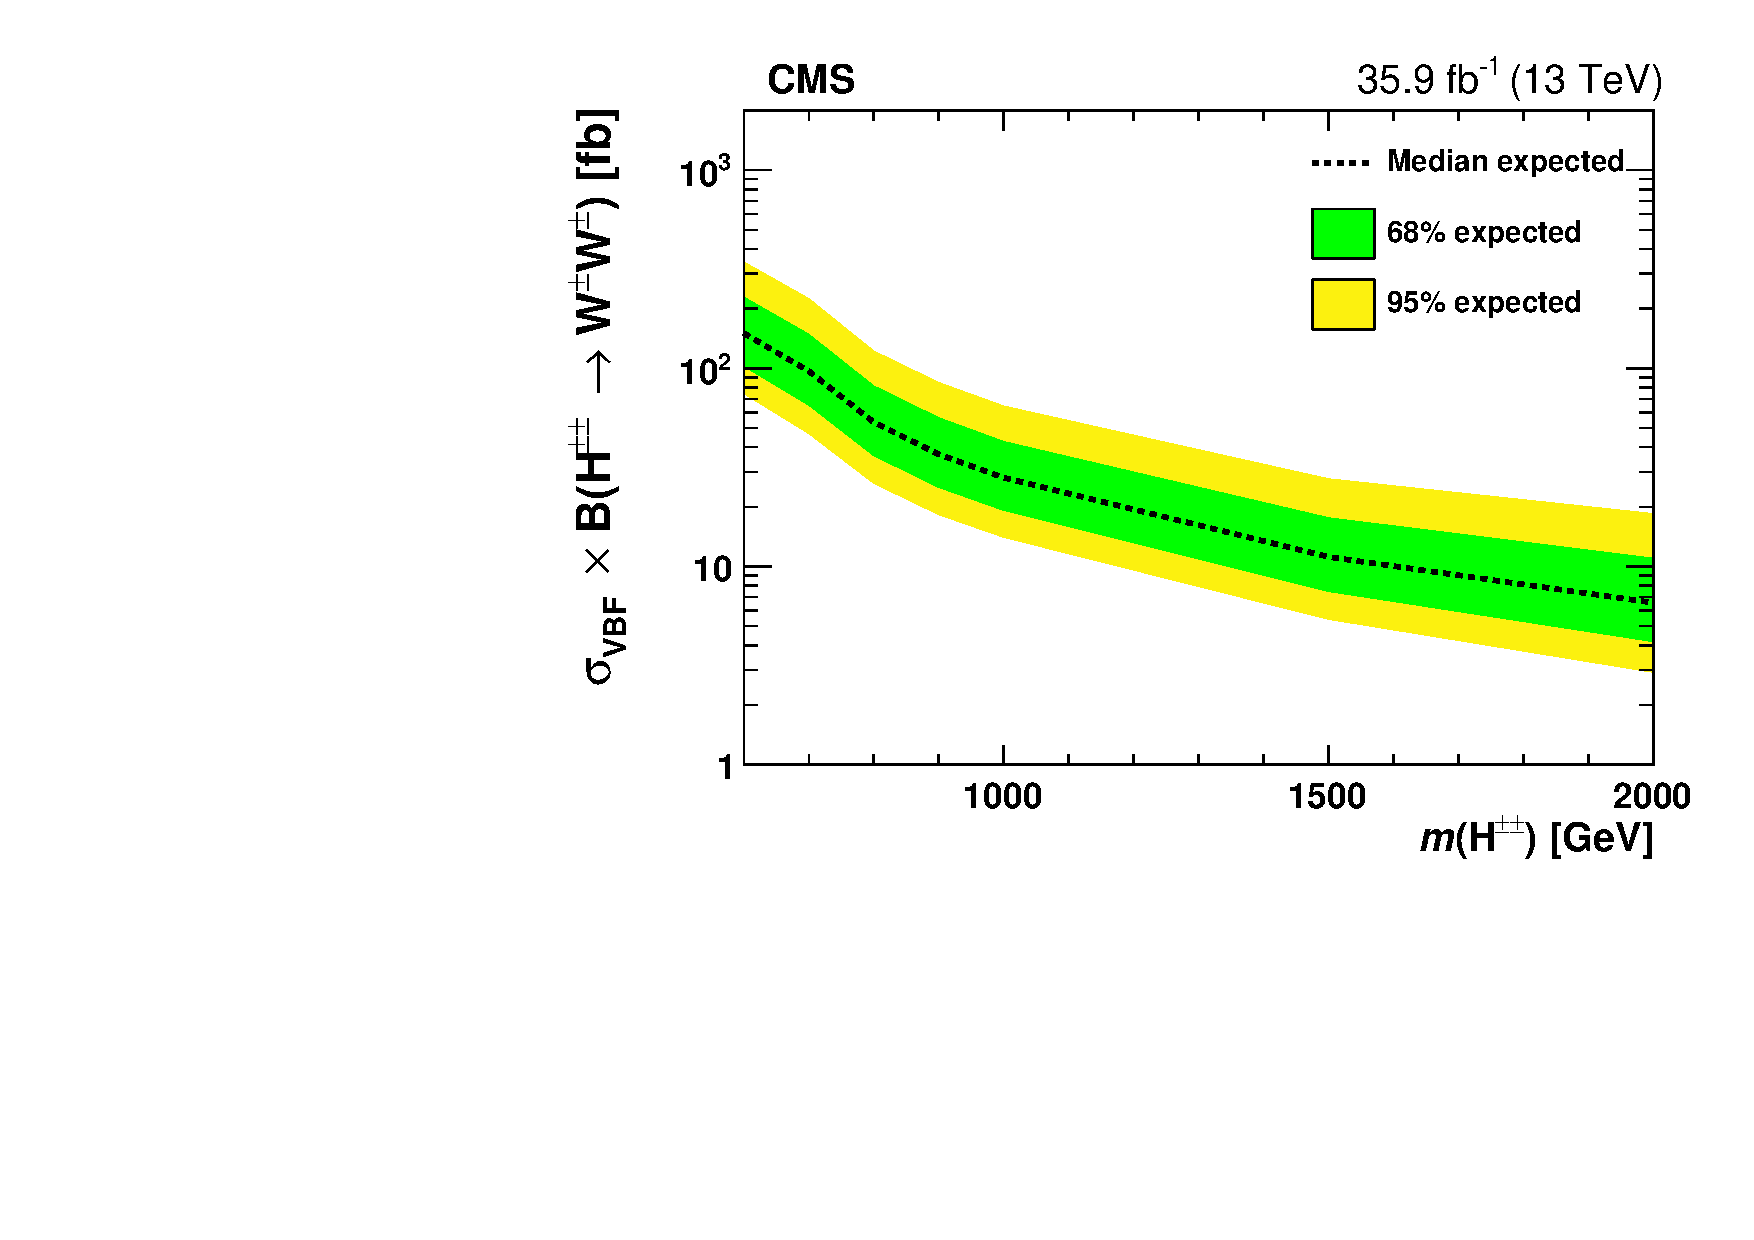
\includegraphics[width=0.45\textwidth]{Plots/plots/limits_wpwp.pdf}
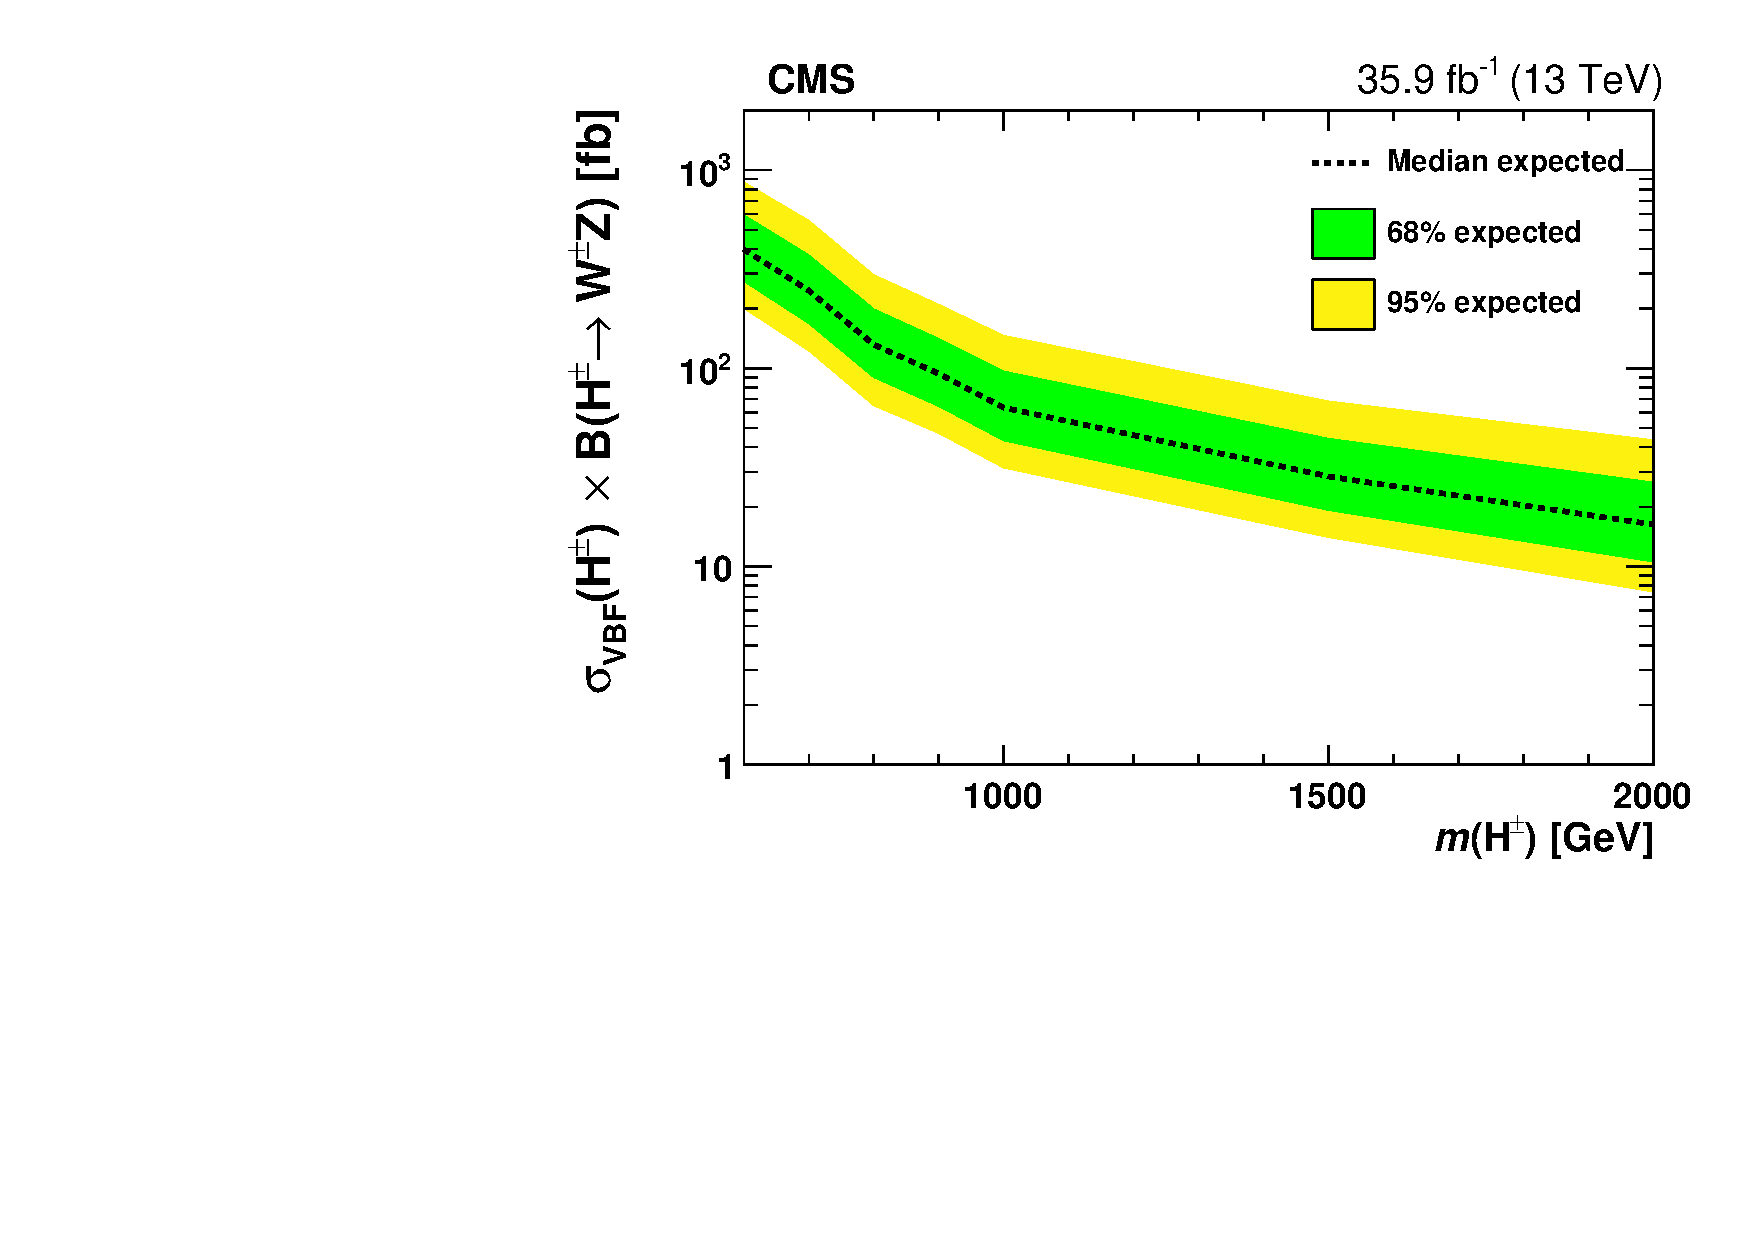
\includegraphics[width=0.45\textwidth]{Plots/plots/limits_wpz_lnu.pdf}
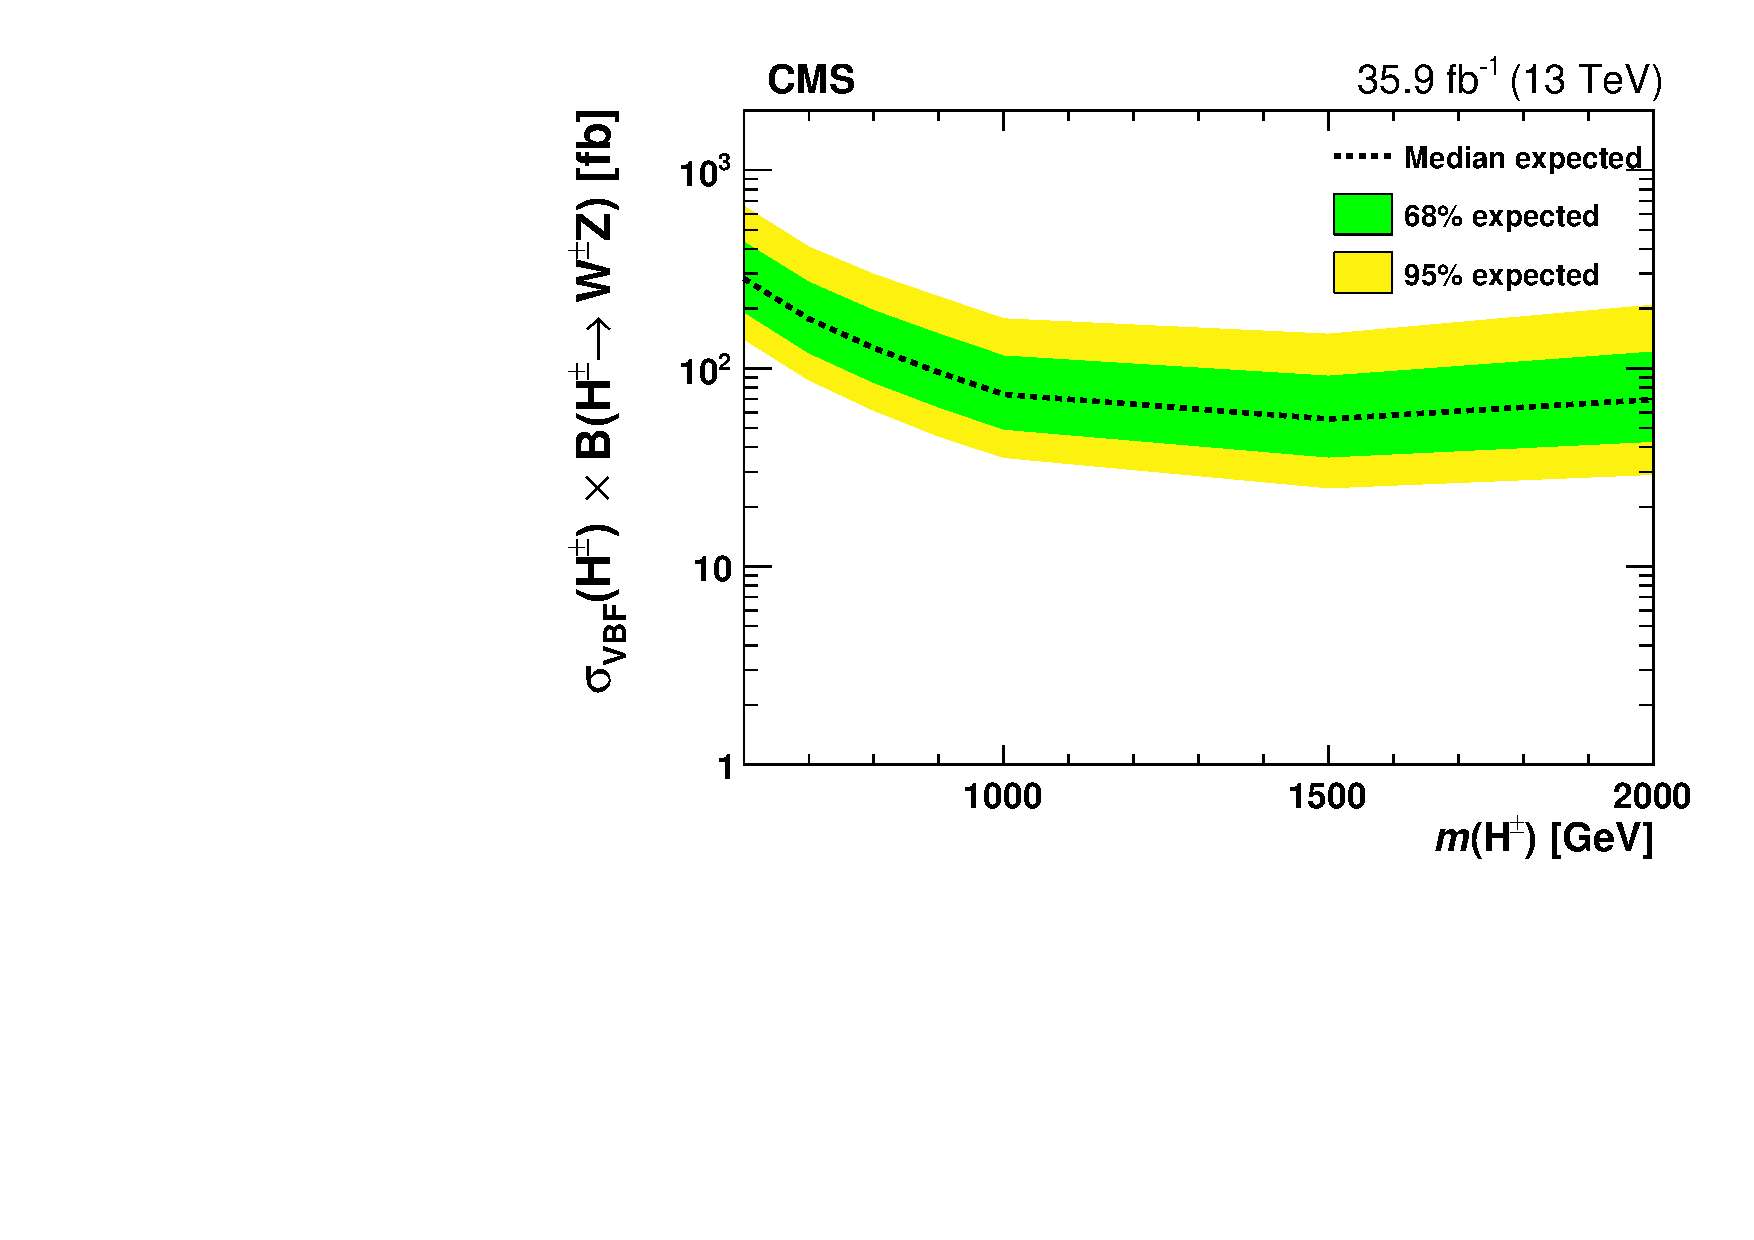
\includegraphics[width=0.45\textwidth]{Plots/plots/limits_wpz_ll.pdf}
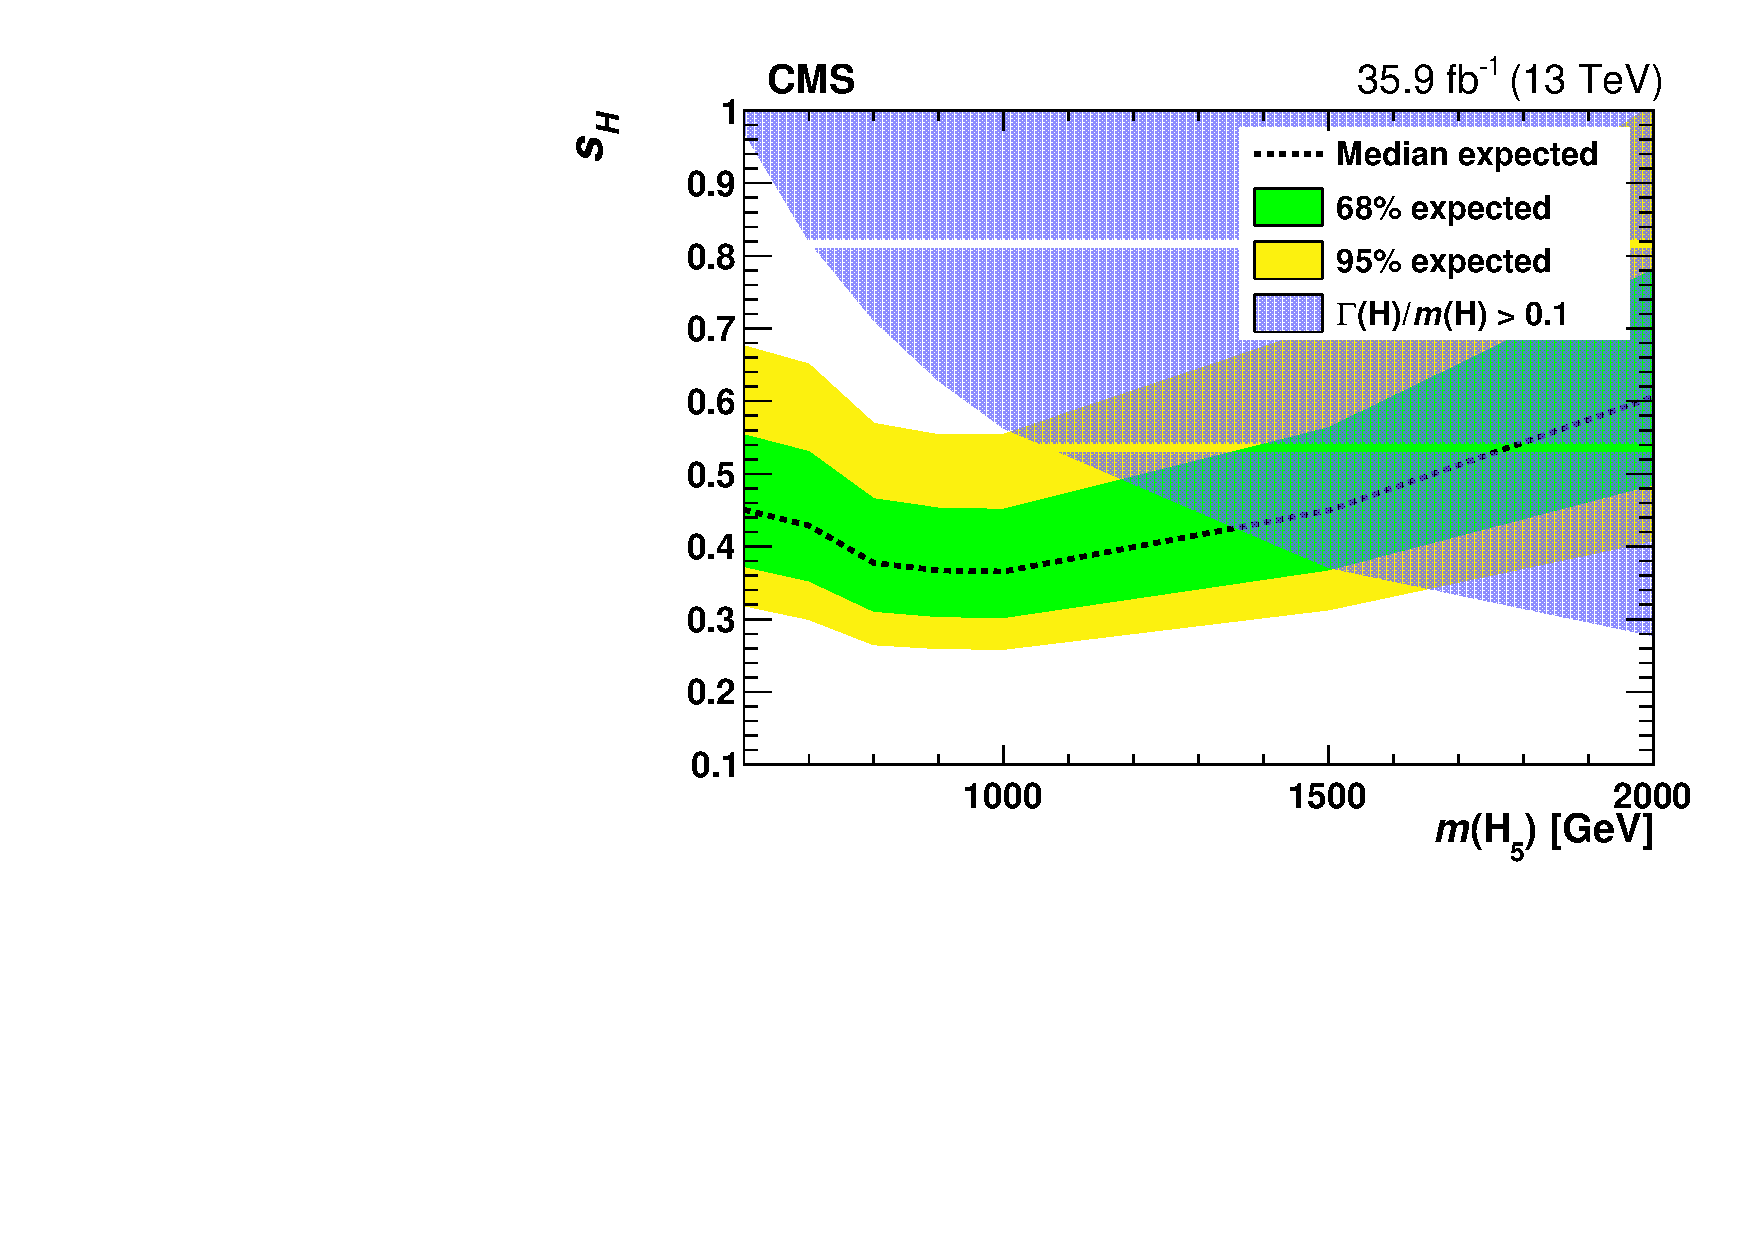
\includegraphics[width=0.45\textwidth]{Plots/plots/limits_model.pdf}
\caption{Expected and observed exclusion limits at 95\% confidence level as functions of $m(\PHpmpm)$ and $m(\PHpm)$ for $\sigma_\mathrm{VBF}(\PHpmpm) \, \mathcal{B}(\PHpmpm\to \PW\PW)$ (top left) and $\sigma_\mathrm{VBF}(\PHpm) \, \mathcal{B}(\PHpm\to \PW\Z)$ in the  $\PW V$ (top right) and $\PZ V$ (bottom left) final states, and on the ratio of vacuum expectation values in the GM model (bottom right). The blue shaded area covers the theoretically not allowed parameter space~\cite{Zaro:2002500}.
}
\label{fig:limits_s}
\end{figure}
% \section{Future Prospects} % (fold)%

% section future_prospects (end)
This is just the starting phase of quartic-gauge coupling studies and the VBS. Due to low cross-section of the VBS process, it is not yet probed. However with the full Run-2 (2016-2018) data collected by the CMS, which corresponds to $\sim$150 $fb^{-1}$. Thus, using the full Run-2 data it will definitly improve the aQGC limits by several factors along with it one might be able to look for the SM electroweak process of $W^+W^-jj$, which should be observed with a significance of at least 2-$\sigma$. The Run-3 of the LHC will be much more exiciting for this kind of studies and it should definitely reflect some information about the EWSB mechanism.




% chapter summary_&_outlook (end)